\documentclass[12pt, letterpaper]{article}
\usepackage[utf8]{inputenc}
\usepackage{graphicx}
\usepackage{floatrow}
\usepackage{multicol}
\usepackage{csquotes}

\graphicspath{ {./images/}}

\title{Classic Cocktails}
\author{Compiled By Dustin Ryan-Roepsch}

\begin{document}

\maketitle

\pagebreak
\section{Margarita}
The Margarita is one of the most popular cocktails in North America—for good reason.
Combining the tang of lime and the sweetness of orange liqueur with the distinctive strength of 
tequila, the classic Margarita strikes all of the right keys.

\subsection*{Ingredients}

\begin{multicols}{2}

\begin{tabular} { r | l}
    15ml & Lime Juice \\
    20ml & Triple Sec \\
    50ml & Tequila \\
    pinch & Salt
\end{tabular}

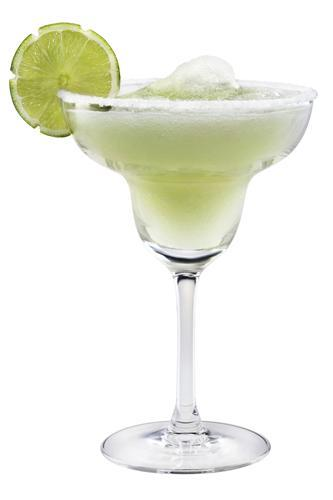
\includegraphics[height=6cm]{margarita}

\end{multicols}


\subsection*{Method}
Rim the edge of a cocktail glass with salt by coating the edge with lime juice and dipping into the salt.
Add the other ingredients to a cocktail shaker with a few cubes of ice.
Shake well for 10-15 seconds or until the outside of the shaker becomes frosted.
Strain into a cocktail glass and serve.

\pagebreak
\section{Fitzgerald}
The Fitzgerald was invented by Dale Degroff in the 1990s. Starting in the early 90s at the Rainbow Room,
New York, Mr DeGroff was instrumental in the revival and expansion of the American bar scene.
His advocacy for using fresh juices in drinks helped revitalise bars into using fresh ingredients instead of bottled sweetened juices.

\subsection*{Ingredients}

\begin{multicols}{2}

\begin{tabular} { r | l}
    25ml & Lemon Juice \\
    15ml & Simple Syrup \\
    2 dashes & Angostura Bitter \\
    50ml & Dry Gin
\end{tabular}

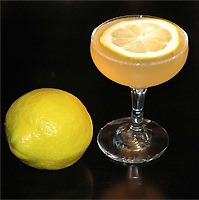
\includegraphics[height=6cm]{fitzgerald}

\end{multicols}


\subsection*{Method}
Add all ingredients to a cocktail shaker with ice and shake well.
Strain into a chilled cocktail glass. Garnish with a lemon wedge and serve.

\pagebreak
\section{Bahia}
This white rum-based crowd pleaser is made with 3 other ingredients: pineapple juice, coconut cream, cream.
\subsection*{Ingredients}

\begin{multicols}{2}

\begin{tabular} { r | l}
    90ml & Pineapple Juice \\
    75ml & White Rum \\
    15ml & Coconut Cream
\end{tabular}

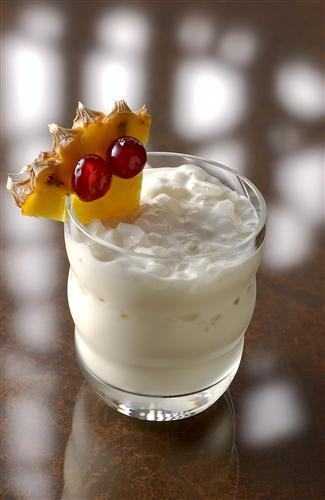
\includegraphics[height=6cm]{bahia}

\end{multicols}

\subsection*{Method}
Add all ingredients to a blender with ice and blend until smooth. Pour into a highball glass.
Garnish with a pineapple wedge, a maraschino cherry and a mint sprig, and serve.

\pagebreak
\section{White Lady}
The original recipe for the White Lady was devised by Harry MacElhone in 1919 at Ciro's Club in London.
He originally used crème de menthe, but replaced it with gin at Harry's New York Bar in Paris in 1929.

\subsection*{Ingredients}

\begin{multicols}{2}

\begin{tabular} { r | l}
    30ml & Triple Sec \\
    20ml & Lemon Juice \\
    40ml & Gin
\end{tabular}

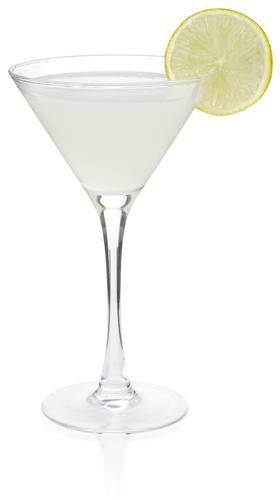
\includegraphics[height=6cm]{whitelady}

\end{multicols}

\subsection*{Method}
Add all ingredients to a cocktail shaker with ice.
Shake well for 10-15 seconds or until the outside of the shaker becomes frosted.
Strain into a chilled cocktail glass and serve.

\pagebreak
\section{Piña Colada}
As the story goes, the Piña Colada debuted in 1952, when it was first mixed by Ramon Marrero Perez,
the head barman at the Caribe Hilton in Old San Juan, Puerto Rico. Perez had blended up a winner,
and the tropical drink enjoyed its place in the sun for decades,
finding its way to American shores and faraway isles.

\subsection*{Ingredients}

\begin{multicols}{2}

\begin{tabular} { r | l}
    50ml & Pineapple Juice \\
    50ml & White Rum \\
    30ml & Coconut Cream
\end{tabular}

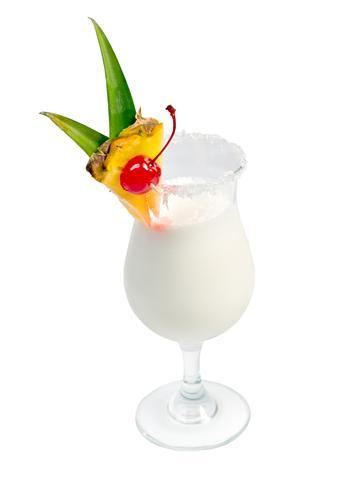
\includegraphics[height=6cm]{pinacolada}

\end{multicols}

\subsection*{Method}
Add all ingredients to a blender with ice and blend until smooth.
Pour into a hurricane glass. Garnish with a slice of pineapple and a cocktail cherry before serving.

\pagebreak
\section{Vodka Martini}
With only 2 essential ingredients, a classic martini is one of the easiest cocktails around.
The martini's simplicity has no bearing on its elegance.
You will feel on top of the world after your first sip.
\subsection*{Ingredients}

\begin{multicols}{2}

\begin{tabular} { r | l}
    60ml & Vodka \\
    10ml & Dry Vermouth 
\end{tabular}

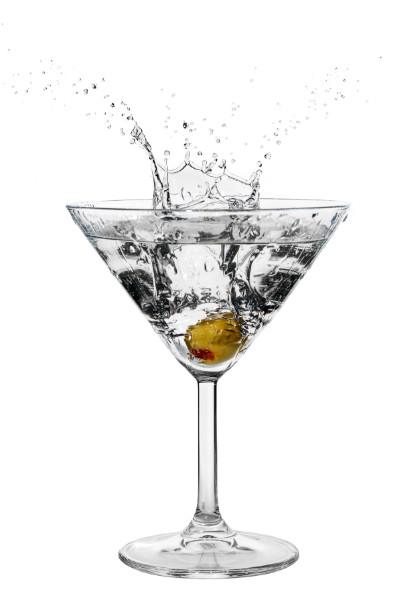
\includegraphics[height=6cm]{vodkamartini}

\end{multicols}

\subsection*{Method}
Add all ingredients to a blender with ice and blend until smooth.
Pour into a hurricane glass. Garnish with a slice of pineapple and a cocktail cherry before serving.

\pagebreak
\section{Daiquiri}
The daiquiri is one of the six basic drinks listed in David A. Embury's classic 
The Fine Art of Mixing Drinks, which also lists some variations
\subsection*{Ingredients}

\begin{multicols}{2}

\begin{tabular} { r | l}
    20ml & Lime Juice \\
    60ml & White Rum  \\
    2 teaspoons & Sugar
\end{tabular}

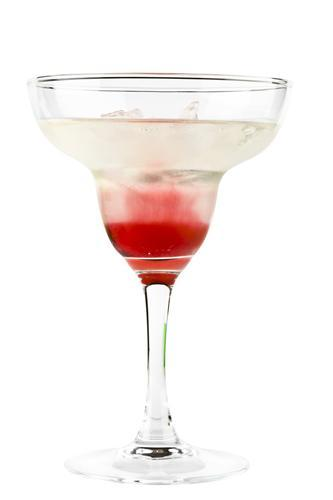
\includegraphics[height=6cm]{daiquiri}

\end{multicols}

\subsection*{Method}
Add all ingredients to a cocktail shaker with ice. Stir well to dissolve the sugar.
Shake well for 10-15 seconds or until the outside of the shaker becomes frosted.
Strain into a chilled cocktail glass and serve.

\pagebreak
\section{Screwdriver}
In the UK, it is referred to as a \enquote{vodka and orange}.
\subsection*{Ingredients}

\begin{multicols}{2}

\begin{tabular} { r | l}
    50ml & Vodka \\
    100ml & Orange Juice  \\
\end{tabular}

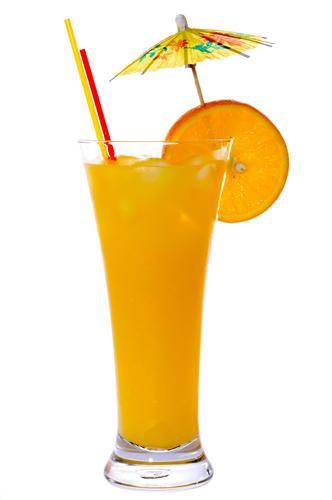
\includegraphics[height=6cm]{screwdriver}

\end{multicols}

\subsection*{Method}
Stir together the vodka and orange juice directly in a highball glass with ice.
Garnish with an orange slice and serve

\pagebreak
\section{Gimlet}
Not the podcast company, The gimlet is a cocktail made of gin and Rose's Lime Juice.
A 1928 description of the drink was: gin, and a spot of lime. 
\subsection*{Ingredients}

\begin{multicols}{2}

\begin{tabular} { r | l}
    15ml & Lime Juice \\
    60ml & Gin  \\
    15ml & Sugar Syrup  \\
\end{tabular}

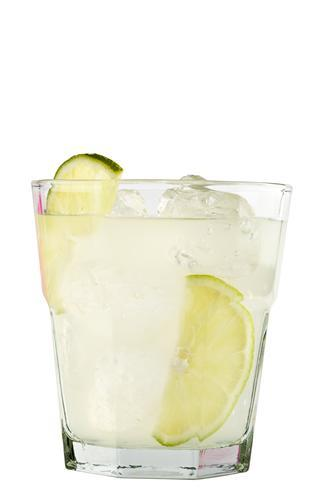
\includegraphics[height=6cm]{gimlet}

\end{multicols}

\subsection*{Method}
Stir together the vodka and orange juice directly in a highball glass with ice.
Garnish with an orange slice and serve

\end{document}